\documentclass[11pt,a4paper]{article}

\usepackage{../../templates/style}

\begin{document}

\begin{problem}{Conquerer}{standard input}{standard output}{1 second}{64 megabytes}

\textit{ผู้ครอบครอง} เป็นเกมตารางที่ได้รับการออกแบบมาเพื่อใช้ในการแข่งขันคอมพิวเตอร์โอลิมปิกในประเทศไทยในปี ๒๕๔๙ โดยเฉพาะ กติกากำหนดให้เล่นบนตารางจัตุรัสขนาด $n\times n$ โดยที่ ด้านบน ด้านขวา ด้านล่าง และ ด้านซ้ายคือ ทิศเหนือ \textbf{(N)} ทิศตะวันออก \textbf{(E)} ทิศใต้ \textbf{(S)} และทิศตะวันตก \textbf{(W)} ตามลำดับ ผู้เล่นจะยืนอยู่สี่คน โดยแต่ละคนจะอยู่ที่มุมกระดานทั้งสี่ โดยคนแรกจะอยู่ที่มุมของด้านเหนือกับตะวันออก คนถัดไปอยู่ที่มุมเวียนตามเข็มนาฬิกา และคนที่สี่จะอยู่มุมของด้านทิศเหนือติดกับทิศตะวันตก ผู้เล่นจะเวียนกันเดินตั้งแต่คนที่หนึ่งจนถึงคนที่สี่ แล้วเวียนกลับมาคนที่หนึ่งใหม่ไปเรื่อยๆ ผู้เล่นแต่ละคนสามารถเคลื่อนที่ไปในตารางได้เฉพาะช่องหนึ่งช่องที่ติดกันกับที่ยืนอยู่โดยการเคลื่อนที่จะระบุตามทิศใดทิศหนึ่ง (เหนือ ตะวันออก ใต้ หรือ ตะวันตก) ถ้าหากผู้เข้าแข่งขันคนใดพยายามเดินออกนอกตารางในแต่ละด้านหรือเดินไปยังพื้นที่ที่ผู้อื่นกำลังยืนอยู่ ผู้เข้าแข่งขันคนนั้นจะต้องยืนอยู่ที่เดิม เจ้าของพื้นที่ในแต่ละช่องคือผู้ที่ยืนอยู่บนช่องนั้นหรือเป็นคนที่เดินผ่านช่องนั้นหลังสุด เมื่อผู้เล่นเดินจนครบแล้วทุกช่องในกระดานยังถูกครอบครองไม่ครบให้ถือว่าไม่มีการแพ้ชนะเกิดขึ้น ผู้ชนะคือผู้ที่มีพื้นที่ครอบครองสูงที่สุด ทั้งนี้เป็นไปได้ที่จะมีผู้ชนะมากกว่าหนึ่งคน
\bigskip

\textbf{ตัวอย่าง}

กำหนดให้ผู้เล่นมีทิศทางเดินตามที่กำหนด

\begin{tabular}{cc}
ผู้เล่น	&ทิศทาง\\
1	&SE\\
2	&WW\\
3	&NN\\
4	&ES\\
\end{tabular}

ผลที่ได้ของการครอบครองจะเป็นดังลำดับด้านล่าง ทั้งนี้หมายเลขในตารางจะระบุหมายเลขของผู้ครอบครอง และหมายเลขที่ขีดเส้นใต้คือตำแหน่งที่ผู้เล่นหมายเลขนั้นยืนอยู่

\begin{figure}[h]
\centering
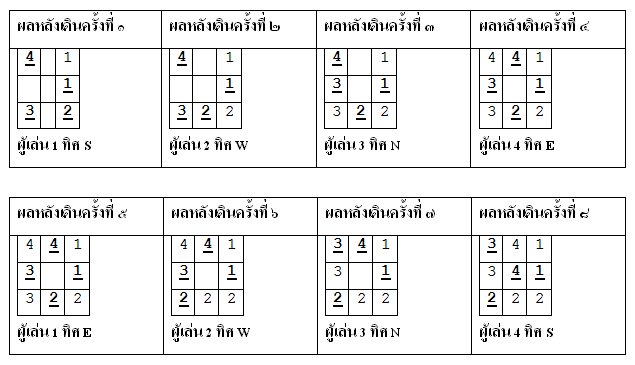
\includegraphics[width=0.7\textwidth]{../latex/img/1033/1033-1.png}
\end{figure}
สรุปได้ว่าผู้เล่นหมายเลข 2 เป็นผู้ชนะเพราะครอบครองได้มากที่สุด คือ 3 ช่อง

\bigskip
\underline{\textbf{โจทย์}}  จงเขียนโปรแกรมเพื่อรับข้อมูลทิศทางการเดินของผู้เล่นแต่ละคน แล้วหาว่าจากข้อมูลดังกล่าวมีผลของการแพ้ชนะหรือไม่ ถ้าหากมีให้ระบุว่ามีใครบ้างที่เป็นผู้ชนะ

\InputFile

\textbf{บรรทัดแรก} รับค่าจำนวนเต็ม $n$ $k$ แทนข้อมูลขนาดของตาราง $(3 \leq n \leq 100)$ และจำนวนก้าวที่ผู้เล่นทุกคนเดิน $(2 \leq k \leq 1\,000)$

\textbf{บรรทัดที่ $2$ ถึง $4k+1$} ในบรรทัดที่ $4(i-1) + m + 1$ จะเป็นข้อมูลการเดินครั้งที่ $m$ ของผู้เล่นคนที่ $i$ โดยที่ทิศทางการเดินจะเป็น ‘N’ ‘E’ ‘S’ หรือ ‘W’ ซึ่งหมายถึงทิศเหนือ ตะวันออก ใต้ และ ตะวันตก ตามลำดับ

\OutputFile

ให้แสดงผลตามเงื่อนไขต่อไปนี้
\begin{itemize}

\item ถ้าหากเดินไปจนหมดข้อมูลที่ให้มาแล้วไม่มีผู้ชนะ ให้แสดง 'No' ในบรรทัดแรก เท่านั้น
\item ถ้าหากมีผู้ชนะเกิดขึ้นให้ระบุว่า ผู้ชนะมีทั้งหมดกี่คน ด้วยพื้นที่เท่าใด และมีหมายเลขใดบ้าง โดยบรรทัดแรกจะมีจำนวนเต็มสองจำนวนคั่นด้วยช่องว่างคือจำนวนผู้ชนะ $x$ และจำนวนช่องของพื้นที่ที่ผู้ชนะได้ครอบครอง จากนั้น $x$ บรรทัดมีจำนวนเต็มอยู่หนึ่งค่าซึ่งเป็นหมายเลขของผู้ชนะ โดยเรียงลำดับจากน้อยไปมาก
\end{itemize}

\Examples

\begin{example}
\exmp{3 2
S
E
W
W
N
N
E
S}{1 3
2}%
\end{example}


\Source

การสอบแข่งขันคณิตศาสตร์และวิทยาศาสตร์โอลิมปิกแห่งประเทศไทย
ประจำปี พ.ศ.2549 (สอบแข่งขันรอบที่ 2 ภาคปฏิบัติวันที่ 2)

\end{problem}

\end{document}